\section{Convolutional Neural Networks applications} \label{sec:cnn}

Convolutional neural network (CNN or ConvNet) is a class of deep neural networks often applied to analyzing visual imagery. CNN is based on multi-layer neural networks that learn relevant features from images using filters, performing several tasks like object classification, detection, and segmentation. Concretely, early versions of CNN are good at classifying handwritten digits, fruits, animals, etc. Commonly, CNN is made up of three types of layer: Convolution layer, Pooling layer, and Fully-connected layer. 

\begin{figure} [H]
    \centering
    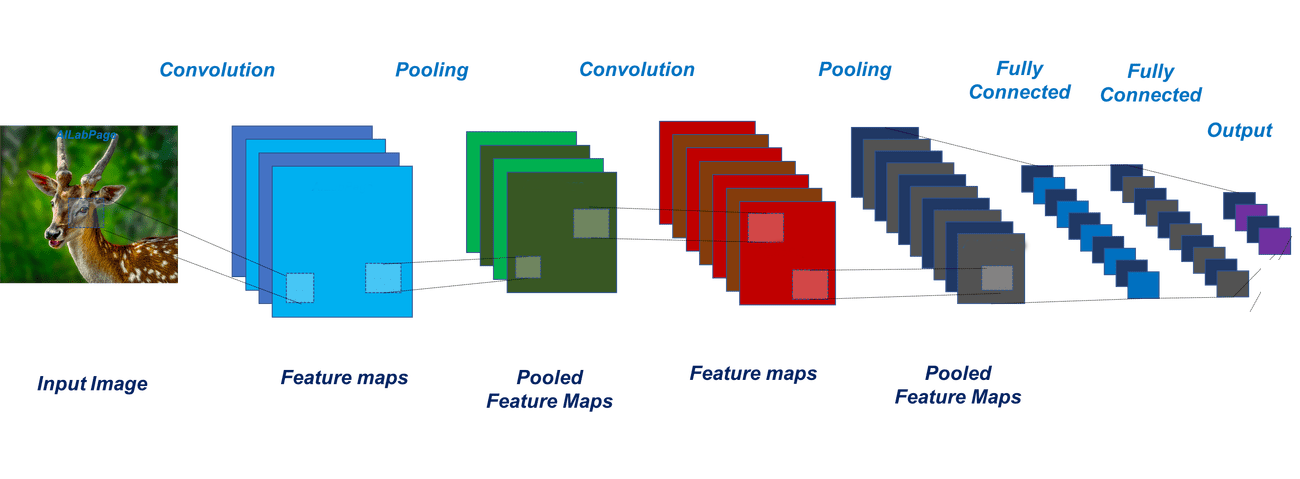
\includegraphics[width=0.9\textwidth]{chapter2/image/CNN.png}
    \caption{General architecture of CNN}
    \label{fig:cnn}
\end{figure}

Some popular architectures in the field of CNN are VGG \cite{vgg}, ResNet \cite{resnet}. Although they have a high accuracy score in computer vision tasks, they fail to run on mobile devices as they have high latency. Next in this section, some models that are capable of running on mobile phones are presented. I divide them according to tasks: object classification, object detection, and object classification.

\subsection{Object classification}
Object classification involves taking an input image and outputting a class that the image falls under. \textbf{Figure \ref{fig:cnn}} is an example of a classification network, where animals are classified. Head of classification models usually consists of fully-connected layers. The number of classes is often equal to the number of neural at the last layer. \par

Some popular image classification models are ResNet, Inception, PyramidNet. However, they require heavy computational resources, are often run on GPU. Models deployed on mobile devices often have simpler architecture and smaller size. Some of them are MobiNetv2 \cite{mobilenetv2}, MobiDets \cite{mobiledets}. These models have been used for some applications on smartphones like flower classification, food classification.


\subsection{Object detection}
Object detection aims at identifying objects of interest in images. Existing models can be categorized into two-stage detectors and one-stage single shot
detectors. For two-stage detectors, including R-FCN, ThunderNet \cite{thundernet}, region proposals must be generated first before the detector can make any subsequent predictions. Two-stage detectors are not efficient in the inference phase due to this multi-stage nature. 

On the other hand, one-stage single shot detectors, such as SqueezeDet \cite{squeezenet}, SSD, YOLO, require only one single pass through the network to predict all the bounding boxes, making them ideal candidates for efficient inference on edge devices. Among them, SSDLite is an efficient variant of SSD that has become one of the most popular lightweight detectors on the smartphone. 

\begin{figure} [H]
    \centering
    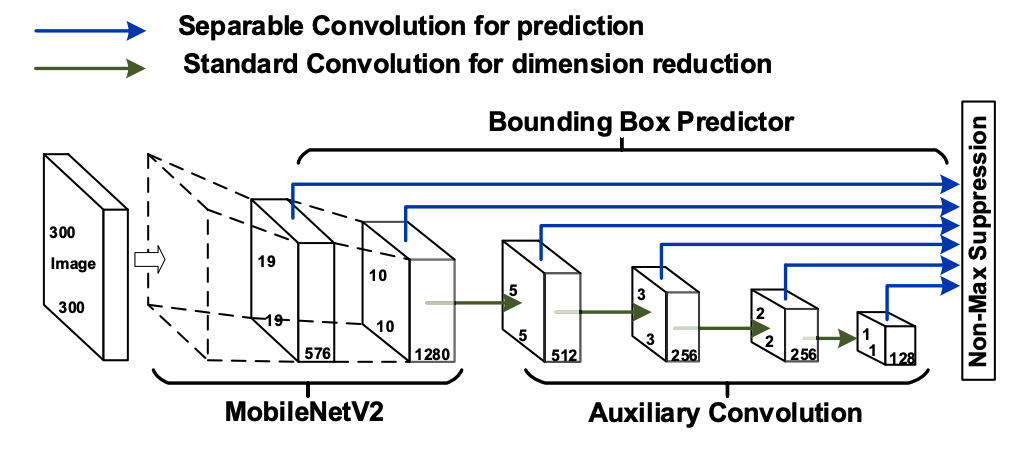
\includegraphics[width=0.9\textwidth]{chapter2/image/ssdlite.png}
    \caption{The network architecture of MobilNetV2-SSDLite}
    \label{fig:cnn}
\end{figure}

SSDLite is a general-purpose model; some applications of it are license plate detection, car detection, face detection, hand detection, to name but a few.

\subsection{Object segmentation}
ConvNets are widely used for segmentation problem, which is already introduced in \textbf{section \ref{sec:pb}}. Most modern models for segmentation are composed of two components: upsampling and downsampling. \par
\begin{figure} [H]
    \centering
    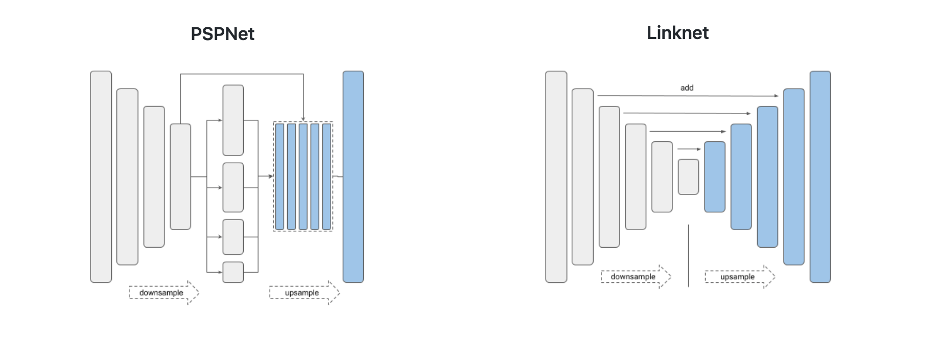
\includegraphics[width=0.9\textwidth]{chapter2/image/segnet.png}
    \caption{Architecture of modern segmentation models}
    \label{fig:my_label}
\end{figure}
While upsampling encodes the input image into feature representations at multiple levels, downsampling is to restore the condensed feature map to the original size of the input image. There are many semantic segmentation networks that have high accuracy such as Mask R-CNN \cite{maskrcnn}, SegNet\cite{segnet}, PSPNet\cite{pspnet}, but poor about speed. For instance, PSPNet which uses pyramid pooling module for more reliable prediction has 65.7 million parameters and runs at about 1 FPS.  \par

Recent approach for the task of object segmentation is \textbf{DeepLabv3+} - an extension of DeepLabv3 in encoder-decoder structure. In general, DeepLabv3 is used as an encoder. The encoder module encodes multi-scale contextual information by applying atrous convolution at multiple scales. This architecture is able to perform several parallel atrus convolution with different rates. Meanwhile, the decoder module refines the segmentation results along object boundaries. \par

\begin{figure} [H]
    \centering
    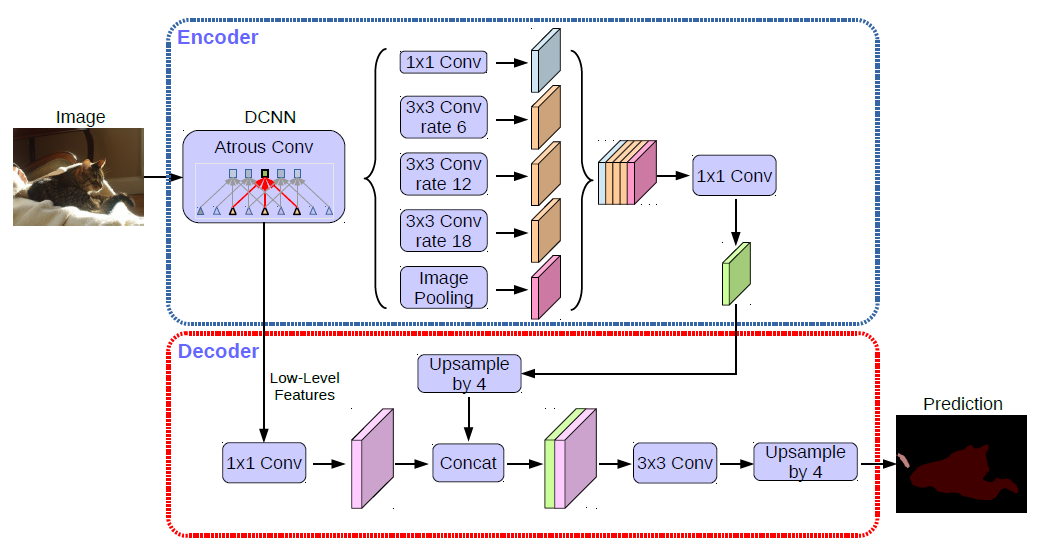
\includegraphics[width=0.8\textwidth]{chapter2/image/deeplab.png}
    \caption{DeepLabv3+ architecture for segmentic segmentation. Source \cite{deeplabv3plus}}
    \label{fig:my_label}
\end{figure}

In fact, applications of segmentation models on smartphones are manifold, ranging from road scene segmentation to human segmentation to style transfer. In the next chapter, I will propose a lightweight segmentation model that aims to recognize hair and clothes. \par



